% !TeX program = lualatex
% !TeX root = luaking.tex
% !TeX encoding = UTF-8
% !TeX spellcheck = cs_CZ
%---------------------------------------------------------------------------------------------------
% file fey1ch19.tex
%---------------------------------------------------------------------------------------------------
%=========================== Kapitola: Hmotný střed; Moment setrvačnosti ==========================
\setchaptertoc
\chapter{Hmotný střed; Moment setrvačnosti}\label{fyz:IchapXIX}
  \section{Vlastnosti hmotného středu}\label{fyz:IchapXIXsecI}
    V přecházející kapitole jsme zjistili, že, působí-li velmi mnoho sil na složitou soustavu
    částic, ať už jde o tuhé těleso, pružné těleso, hvězdný oblak nebo něco jiného, a sečteme-li
    všechny tyto síly (jsou to samozřejmě vnější síly, neboť vnitřní síly se vzájemně vyrušily) a
    díváme se na celý soubor částic jako na jedno těleso s celkovou hmotností \(M\), pak „uvnitř“
    existuje takový bod - hmotný střed (\emph{těžiště}) -, že výslednice vnějších sil působí taková
    zrychlení tohoto bodu, jakoby v něm byla soustředěna celá hmotnost souboru. Zabývejme se nyní
    hmotným středem trochu podrobněji.
    
    Poloha hmotného středu (ve zkratce \(T\)) je určena rovnicí
    \begin{equation}\label{fyz:eq739}
      \vec{R}_{CM}=\frac{∑m_ir_i}{∑m_i}.
    \end{equation}
    To je, jak je vidět, vektorová rovnice, která ve skutečnosti představuje tři rovnice (jednu pro
    každou ze tří souřadnic). Budeme se zabývat jen jednou, \(x\)-ovou souřadnicí, neboť
    porozumíme-li vztahům pro jednu souřadnicí, snadno je přeneseme na další dvě. Co znamená výraz
    \begin{equation}\label{fyz:eq740}
      X_{CM}=\frac{∑m_ix_i}{∑m_i}
    \end{equation}
    Předpokládejme, že těleso je rozděleno na malé části, z nichž každá má stejnou hmotnost \(m\).
    Celková hmotnost je pak rovna počtu částí \(N\) násobenému hmotností jednotlivé části. Tato
    rovnice pak znamená, že máme sčítat všechny polohy \(x_i\) a vydělit je počtem částí
    \begin{equation}\label{fyz:eq743}
      X_{CM} =  \frac{m∑x_i}{mN}= \frac{∑xi}{N}.
    \end{equation}
    
    \begin{figure}[ht!] %\ref{fyz:fig402}
      \centering
      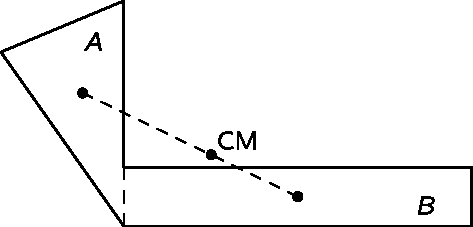
\includegraphics[width=0.8\linewidth]{fyz_fig402.pdf}
      \caption{Hmotný střed složeného tělesa leží na přímce spojující hmotné středy obou částí
              (\cite[s.~260]{Feynman01})}
      \label{fyz:fig402}
    \end{figure}

    Takže \(X_{CM}\) je střední hodnota všech \(x_i\) jsou-li všechny hmotnosti \(m_i\) stejné.
    Předpokládejme však, že některá část by byla dvakrát těžší než ostatní, pak by se příslušné
    \(x\) vyskytlo v součtu dvakrát To lze snadno pochopit, neboť tuto část s dvojnásobnou hmotností
    si můžeme představit rozdělenou na dvě poloviny, které jsou stejně těžké jako ostatní části. Při
    počítání průměru musíme příslušné \(x\) započítat dvakrát, neboť tam jsou takové části dvě.
    Takže \(X\) je průměrná poloha všech částí ve směru osy \(x\), přičemž poloha každé části se
    musí započítat úměrně ke své hmotnosti. Z toho lze snadno dokázat, že \(X\) musí ležet někde
    mezi největším a nejmenším \(x\), a proto leží uvnitř obalu ohraničujícího celé těleso. Nemusí
    se nacházet uvnitř materiálu samotného tělesa, neboť těleso může mít například tvar kružnice,
    jako prsten, kde hmotný střed je ve středu prstenu, a ne v samotném prstenu.

    Je-li těleso symetrické, například obdélník a má nějakou rovinu symetrie, pak hmotný střed leží
    někde v této rovině. V případě obdélníka existují dvě takové roviny, čímž je poloha hmotného
    středu určena jednoznačně. Jde-li o libovolné symetrické těleso, pak jeho hmotný střed leží
    někde na ose symetrie, neboť v takovém případě existuje stejný počet kladných i záporných \(x\).

    Všimněme si i dalšího zajímavého případu. Předpokládejme, že máme těleso složené ze dvou částí
    \(A\) a \(B\) (obr. \ref{fyz:fig402}). Hmotný střed celého tělesa pak lze vypočítat takovýmto
    způsobem: Nejdříve najdeme hmotný střed části \(A\), potom části \(B\) a zjistíme i hmotnost
    každé části \(M_A\) a \(M_B\). Pak budeme uvažovat nový problém, kdy hmota o hmotnosti \(M_A\)
    je soustředěna v bodě, jenž je hmotným středem \(A\), a hmota o hmotnosti \(M_B\) v bodě, jímž
    je hmotný střed tělesa \(B\). Hmotný střed těchto dvou hmotných bodů je pak hmotným středem
    celého tělesa. Jinak řečeno, jestliže jsme našli hmotný střed různých částí tělesa, nemusíme při
    výpočtu hmotného středu celého tělesa začínat úplně znova; stačí, když spojíme jednotlivé části,
    přičemž každou považujeme za hmotný bod umístěný v hmotném středu příslušné části. Podívejme se,
    proč je tomu tak. Předpokládejme, že chceme vypočítat hmotný střed celého tělesa, jehož dvě
    části patří k tělesu \(A\) a některé k tělesu \(B\). Celkovou sumu \(∑m_ix_i\) pak lze rozdělit
    na dvě části - sumu \(∑_Am_ix_i\) týkající se pouze tělesa \(A\) a sumu \(∑_Bm_ix_i\) vztahující
    se pouze k tělesu \(B\). Kdybychom počítali hmotný střed pouze tělesa \(A\), použili bychom
    první sumu, přičemž víme, že ta je rovna \(M_AX_A\) (celková hmotnost částí tělesa \(A\) krát
    poloha hmotného středu tělesa \(A\)) podle věty o hmotném středu aplikované na objekt \(A\).
    Rovněž pro těleso \(B\) máme \(M_BX_B\) a samozřejmě, že sečtením obou máme
    \begin{equation}\label{fyz:eq741}
      MX_{CM}=∑_Am_ix_i+∑_Bm_ix_i=M_AX_A+M_BX_B.
    \end{equation}

    Protože je jasné, že \(M\) je rovno součtu \(M_A\) a \(M_B\), vidíme, že rovnici
    (\ref{fyz:eq741}) lze interpretovat jako zvláštní případ vztahu pro výpočet hmotného středu dvou
    bodových těles, jednoho s hmotností \(M_A\) umístěného v bodě \(X_A\) a druhého s hmotností
    \(M_B\) v bodě \(X_B\).

    Věta o pohybu hmotného středu je velmi zajímavá a měla důležitou úlohu v rozvoji našeho chápání
    fyziky. Předpokládejme, že Newtonův zákon platí pro malé části mnohem většího tělesa. Pak podle
    této věty platí Newtonův zákon i pro větší těleso, ačkoli těleso neznáme detailně. Známe jen
    celkovou sílu, jež na něj působí a jeho hmotnost. Jinými slovy, Newtonův zákon má tu zvláštní
    vlastnost, že platí-li v určitém malém měřítku, bude platit i ve větším měřítku. Nebudeme-li
    míček považovat za velmi složitou věc skládající se z miliard interagujících částic a všimneme
    si pouze pohybu těžiště a vnějších sil působících na míček, zjistíme, že \(\vec{F}= m\vec{a}\),
    kde \(\vec{F}\) je vnější síla působící na míček, \(m\) je jeho hmotnost a \(\vec{a}\) je
    zrychlení jeho těžiště. Takže \(\vec{F}= m\vec{a}\) je zákon, který reprodukuje sám sebe ve
    větším měřítku. (Mělo by existovat slovo, možná řecké, k pojmenování zákona, který reprodukuje
    sám sebe ve větším měřítku.)

    Samozřejmě lze předpokládat, že zákony objevené jako první budou takové, jež se reprodukují ve
    větším měřítku. Proč? Protože měřítko základních „setrvačníků a koleček“ vesmíru má rozměry
    atomu, což je mnohem jemnější měřítko než nesrovnatelně větší měřítko našich běžných pozorování.
    Proto bychom jako první měli objevit zákony týkající se objektů, jejichž vlastnosti nejsou
    vázány na atomová měřítka. Kdyby se zákony platné pro malá tělesa nereprodukovaly ve větším
    měřítku, neobjevili bychom je tak snadno. Jak by to vypadalo, kdyby to bylo obráceně? Musí být
    zákony platné v malém měřítku stejné, jako zákony platné ve větším měřítku? V přírodě samozřejmě
    není nutné, aby zákony na úrovni atomových měřítek musely být stejné, jako zákony na úrovni
    větších měřítek. Předpokládejme, že by pravé zákony pohybu atomů byly dány nějakou podivnou
    rovnicí, která nemá vlastnost, že přejdeme-li k větším měřítkům, zreprodukuje se stejný zákon.
    Ale místo toho má tu vlastnost, že ve větších měřítkách ji lze aproximovat určitým výrazem,
    který když ho rozšíříme dál a dál, bude reprodukovat sám sebe ve větším a větším měřítku. To je
    možné a ve skutečnosti je tomu tak. Newtonovy zákony jsou „chvostem“ atomových zákonů
    extrapolovaných na velmi velké rozměry. Zákony pohybu částic v tom nejjemnějším měřítku jsou
    velmi zvláštní, ale když si vezmeme velké množství částic a složíme je, dostaneme přibližně ale
    jen přibližně, Newtonovy zákony. Newtonovy zákony nám pak umožňují, že můžeme přecházet k větším
    a větším měřítkům, přičemž se zdá, že platí stále stejný zákon. Ve skutečnosti dokonce, jak se
    měřítko zvětšuje, stává se zákon stále přesnějším a přesnějším. Samoreprodukční faktor
    Newtonových rovnic není sice základní vlastností přírody, je však důležitý po historické
    stránce. Základní zákony atomových částic bychom nikdy neobjevili při prvním pozorování, neboť
    první pozorování jsou příliš hrubá. Opravdu se ukazuje, že základní atomové zákony, jež nazýváme
    kvantovou mechanikou, se zcela liší od Newtonových zákonů. Lze je těžko pochopit, neboť všechny
    naše přímé zkušenosti máme s objekty velkých měřítek a chování atomů je zcela jiné než to, co
    vidíme ve velkých měřítkách. Proto nemůžeme říct: „Elektron v atomu je jako planeta obíhající
    kolem Slunce“ nebo něco podobného. Není to jako nic, co známe, protože nic se mu nepodobá. Když
    aplikujeme kvantovou mechaniku na stále větší a větší tělesa, zákony chování mnoha atomů se
    nezreprodukují, ale dostaneme z nich nové zákony - Newtonovy zákony. Ty se potom reprodukují
    počínaje řekněme měřítkem milióntiny mikrogramu, což již představuje miliardy a miliardy atomů,
    až k rozměrům Země a dále. 
    
    Nyní se vraťme k hmotnému středu. Často se nazývá i těžištěm, a to proto, že ve většině případů
    je gravitační pole stejnorodé. Předpokládejme, že máme dostatečně malé rozměry, takže gravitační
    síla není jen úměrná hmotnosti, ale všude je i rovnoběžná s daným směrem. Mějme těleso, na jehož
    všechny části hmoty působí gravitační síly. Nechť mí je hmotnost jedné části. Gravitační síla
    působící na tuto část je pak \(m_i\) krát \(g\). Zůstává otázkou, v kterém bodě máme působit
    jedinou silou tak, abychom vyvážili gravitační sílu působící na těleso a aby se celý objekt
    (jde-li o tuhé těleso) neotáčel? Odpověď je, že síla musí procházet hmotným středem. Dokážeme
    to: Aby se těleso neotáčelo, musí se součet momentů všech sil rovnat nule, neboť kde je moment
    síly, tam je i změna momentu hybnosti, tedy rotace. Proto musíme spočítat momenty sil působící
    na všechny částice a zjistit, jak velký je výsledný moment síly vzhledem k nějaké ose (když osa
    prochází hmotným středem, měl by být nulový). Když budeme \(x\) měřit horizontálně a \(y\)
    vertikálně, budou momenty sil rovny velikostem sil ve směru \(y\), jež vynásobíme velikostí
    příslušného ramene ve směru \(x\) (podle pravidla síla krát rameno síly vzhledem k ose, vůči níž
    určujeme moment síly). Celkový moment síly je roven součtu
    \begin{equation}\label{fyz:eq742}
      τ=∑m_igx_i=g∑m_ix_i,
    \end{equation}
    Proto má-li být celkový moment síly roven nule, musí být součet \(∑m_ix_i\) roven nule. Ale
    \(∑m_ix_i=MX_{CM}\), tj. celková hmotnost krát vzdálenost hmotného středu od osy otáčení, proto
    \(x\)-ová vzdálenost hmotného středu od osy otáčení je rovna nule.

    Zkontrolovali jsme výsledek jen pro vzdálenosti ve směru osy \(x\), ale kdybychom použili
    skutečný hmotný střed, bylo by těleso v rovnováze v jakékoli poloze, neboť otočíme-li ho o
    \ang{90}, dostaneme místo \(x\)-ových \(y\)-ové vzdálenosti. Jinými slovy, je-li těleso
    podepřeno v hmotném středu, nepůsobí na něj moment síly, neboť gravitační pole je homogenní. V
    případě, že těleso je tak velké, že se projeví nerovnoběžnost gravitačních sil, pak určit bod, v
    němž je třeba působit rovnovážnou silou, není jednoduché a jeho poloha se trochu vysune z
    hmotného středu. To je důvodem, proč je třeba rozlišovat mezi hmotným středem a těžištěm. Fakt,
    že těleso podepřené přesně v hmotném středu je v rovnováze ve všech polohách, má další zajímavý
    důsledek. Máme-li místo gravitace nepravou sílu vzniklou zrychlením, můžeme přesně stejným
    matematickým postupem najít polohu bodu k upevnění tělesa, aby setrvačná síla způsobená
    zrychlením nepůsobila žádným momentem síly. Předpokládejme, že těleso je nějak upevněno v
    krabici, která se zrychleně pohybuje se vším, co v ní je. Víme, že z hlediska toho, kdo je
    vzhledem ke krabici v relativním klidu, bude v ní působit efektivní síla setrvačnosti. To
    znamená, že aby se nějaké těleso pohybovalo spolu s krabicí, musíme na něj působit silou, aby se
    zrychlovalo. Tato síla je vyvažována „silou setrvačnosti“, jež je nepravou silou a je rovna
    součinu hmotnosti a zrychlení krabice. Pro člověka v krabici je to stejná situace, jako by se
    krabice nacházela v homogenním gravitačním poli, jehož hodnota „\(g\)“ je rovna zrychlení \(a\).
    Proto setrvačná síla způsobená zrychlením tělesa nepůsobí momentem síly vzhledem k hmotnému
    středu.

    Tato skutečnost má velmi zajímavé důsledky. V inerciální soustavě, jež se nezrychluje, je moment
    síly vždy roven rychlosti změny momentu hybnosti, ale vzhledem k ose, která prochází hmotným
    středem tělesa i když se těleso zrychluje, \emph{stále platí}, že moment síly je roven rychlosti
    změny momentu hybnosti. Dokonce i když se hmotný střed zrychluje, můžeme stále zvolit takovou
    osu, konkrétně tu, která jím prochází, aby platila rovnost momentu síly a rychlosti změny
    momentu hybnosti vzhledem k této ose. Proto věta, že moment síly je roven rychlosti změny
    momentu hybnosti, platí ve dvou obecných případech:

    \begin{enumerate}[noitemsep]
      \item pro pevnou osu v inerciálním systému,
      \item pro osu procházející těžištěm - dokonce i když se těleso pohybuje zrychleně.      
    \end{enumerate}

  \section{Poloha hmotného bodu}\label{fyz:IchapXIXsecII}
    Matematická technika výpočtu hmotného středu těles spadá do kurzu matematiky a takovéto problémy
    jsou vhodnými cvičeními v integrálním počtu. I když známe integrální počet, je dobré znát určité
    triky, jež se k výpočtu polohy hmotného středu dají použít. jeden takový trik využívá tzv.
    \textbf{Pappovy věty}. Zní takto: Vezmeme-li si libovolnou uzavřenou plochu v rovině a pohybem
    této plochy v prostoru vytvoříme těleso tak, aby se každý bod plochy pohyboval kolmo k rovině
    plochy, pak objem tohoto tělesa je roven součinu obsahu plochy průřezu tělesa a vzdáleností,
    kterou urazil hmotný střed! Určitě to platí, budeme-li plochou pohybovat přímo, kolmo k rovině
    plochy; ale budeme-li jí pohybovat po kružnici nebo po jiné křivce mohou vznikat velmi zvláštní
    tělesa. V případě zakřivené dráhy se vzdálenější strana posune víc a bližší méně, takže tyto
    efekty se vzájemně vyrovnají. Proto, chceme-li určit polohu hmotného středu rovinné desky
    rovnoměrné hustoty, můžeme si zapamatovat, že objem vytvořený její rotací kolem nějaké osy je
    roven součinu dráhy, kterou projde hmotný střed a obsahu plochy této desky.

    Chceme-li určit hmotný střed pravoúhlého trojúhelníka se základnou \(D\) a výškou \(H\) (obr.
    \ref{fyz:fig403}), můžeme postupovat následujícím způsobem. Představme si osu podél \(H\) a
    otočme kolem ní trojúhelník o \num{360} stupňů. Tím se vytvoří kužel. Hmotný střed o souřadnici
    \(x\) opsal dráhu \(2\pi x\). Plocha, která se pohybovala, je plocha trojúhelníka a má obsah
    \(\frac{1}{2}HD\). Takže dráha hmotného středu krát obsah plochy trojúhelníka je rovna rotačnímu
    objemu, který je \(\frac{1}{3}\pi D^2H\). Takže \((2\pi x) (\frac{1}{2}HD) =\frac{1}{3}\pi
    D^2H\) neboli \(x=D/3\). Podobným způsobem, rotací kolem druhé osy nebo pomocí argumentu
    symetrie, bychom našli \(y=H/3\). Skutečně, těžiště jakéhokoli homogenního trojúhelníka je v
    průsečíku těžnic (spojnic vrcholů se středy protilehlých stran). Nachází se v \(1/3\) délky
    každé těžnice. Rozřežeme-li trojúhelník na množství pásků rovnoběžných se základnou vidíme, že
    těžnice rozpůlí každý pásek, a proto musí těžiště ležet na těžnici!  

    \begin{figure}[ht!] %\ref{fyz:fig403}
      \centering
      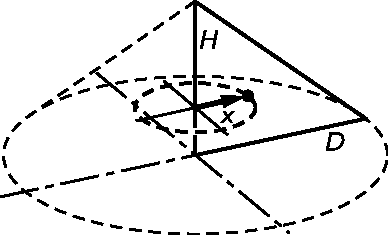
\includegraphics[width=0.8\linewidth]{fyz_fig403.pdf}
      \caption{Pravoúhlý trojúhelník a přímý rotační kužel vytvořený rotujícím trojúhelníkem 
              (\cite[s.~263]{Feynman01})}
      \label{fyz:fig403}
    \end{figure}

    Nyní zkusme komplikovanější příklad. Hledejme hmotný střed homogenního půlkruhového kotouče -
    kotouče rozříznutého na polovinu. Kde se nachází hmotný střed? Hmotný střed celého kotouče je ve
    středu, to je jednoduché, ale pro poloviční, kotouč je situace obtížnější. Nechť \(r\) je
    poloměr a \(x\) nechť je vzdálenost hmotného středu od rovné hrany kotouče. Zatočme jím kolem
    této hrany jako kolem osy a vytvořme kouli. Těžiště se přitom posunulo o \(2\pi x\), obsah
    plochy je \(1/2\pi r^2\) (neboť je to půlkruh). Vytvořený objem je roven \(4/3\pi r^3\), odkud
    máme že
    \begin{align*}
      (2πx)(\frac{1}{2}πr^2)&=\frac{4}{3}πr^3,
      \shortintertext{nebo}
                           x&=\frac{4}{3}rπ.
    \end{align*}

    Existuje další Pappova věta, která je zvláštním případem předcházející věty, takže je rovněž
    pravdivá. Předpokládejme, že místo půlkruhového kotouče bychom měli půlkružnicový drát, v němž
    chceme najít hmotný střed. V tomto případě není hmota ve vnitřní oblasti, pouze v drátu. Ukazuje
    se, že \emph{plocha} vytvořená rotací rovinné křivky je rovna vzdálenosti, o níž se posune
    hmotný střed, vynásobené \emph{délkou} křivky. (Křivku si můžeme představit jako velmi úzkou
    plochu a můžeme použít předcházející větu.)

  \section{Určení momentu setrvačnosti}\label{fyz:IchapXIXsecIII}
    Nyní se věnujme problému určení \textbf{momentu setrvačnosti} různých těles. Vzorec pro výpočet
    momentu setrvačnosti kolem osy \(z\) je 
    \begin{align}
      I&=∑m_i(x^2i+y^2i)  \nonumber \\
      \shortintertext{nebo}
      I&=∫(x^2+y^2)\dl m = ∫(x^2+y^2)ρ\dl V. \label{fyz:eq744}
    \end{align}
    To znamená, že musíme sečíst hmotnosti, z nichž každá je vynásobena druhou mocninou své
    vzdálenosti od osy. Všimněme si, že tu nevystupuje trojrozměrná vzdálenost, ale druhá mocnina
    dvojrozměrné vzdálenosti, ačkoli jde o trojrozměrné těleso. Většinou se omezíme na dvojrozměrné
    objekty, ale vzorec pro rotaci kolem osy \(z\) je stejný jako v trojrozměrném případě.

    \begin{figure}[ht!] %\ref{fyz:fig404}
      \centering
      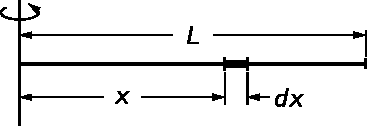
\includegraphics[width=0.8\linewidth]{fyz_fig404.pdf}
      \caption{Přímá tyč \(L\) rotující kolem osy procházející jedním koncem
              (\cite[s.~264]{Feynman01})}
      \label{fyz:fig404}
    \end{figure}

    Jako jednoduchý příklad si představme tyč rotující kolem kolmé osy procházející jejím jedním
    koncem  (obr. \ref{fyz:fig404}). Je třeba sečíst všechny hmotnosti vynásobené druhou mocninou
    \(x\)-ové vzdálenosti (všechny vzdálenosti \(y\) jsou v tomto případě rovny nule). „Součtem“
    máme samozřejmě na mysli integrál z \(x^2\) krát malé elementy hmotnosti. Rozdělíme-li tyč na
    malé elementy délky \(\dl x\), a je-li délka celé tyče \(L\) a její hmotnost \(M\), pak
    \begin{equation*}
      \dl m =\frac{M}{L}\dl x 
    \end{equation*}
    a také
    \begin{equation}\label{fyz:eq745}
      I =∫^L_0x^2\frac{M}{L}\dl x = \frac{M}{L}∫^L_0x^2\dl x=\frac{ML^2}{3}. 
    \end{equation}

    Rozměry momentu setrvačnosti jsou vždy hmotnost krát druhá mocnina délky, takže všechno, co jsme
    skutečně potřebovali zjistit, byl koeficient \(1/3\).

    Čemu je rovno \(I\), prochází-li osa rotace středem tyče? Znovu bychom mohli počítat tento
    integrál, přičemž \(x\) by se měnilo od \(- 1/2 L\) do \(+ 1/2 L\). Všimněme si však několika
    vlastností momentu setrvačnosti. Celou tyč si můžeme představit jako by byla složena ze dvou
    tyčí, každé o hmotnosti \(M/2\) a délce \(L/2\). Momenty setrvačnosti těchto dvou malých tyčí
    jsou stejné a oba jsou dány vzorcem. Proto moment setrvačnosti celé tyče je
    \begin{equation}\label{fyz:eq747}
      I=\dfrac{2\left(\dfrac{M}{2}\right)\left(\dfrac{L}{2}\right)^2}{3} = \dfrac{ML^2}{12}.
    \end{equation}
    Takže je mnohem snadnější točit tyč kolem jejího středu než kolem jejího konce.
    
    Mohli bychom pokračovat ve výpočtech momentu setrvačnosti pro různá jiná zajímavá tělesa. I když
    takové výpočty tvoří část důležitých cvičení v integrálním počtu, nejsou pro nás v podstatě
    zajímavé. Existuje však zajímavá věta, která je velmi užitečná. Předpokládejme, že máme nějaké
    těleso a chceme vypočítat jeho moment setrvačnosti vzhledem k nějaké ose. To znamená, že chceme
    určit setrvačnost, kterou musíme překonat při rotaci kolem této osy. Upevníme-li těleso v
    těžišti na čepu tak, aby se při oběhu kolem osy samo neotáčelo (setrvačně síly nebudou vyvolávat
    žádný moment síly), pak síly potřebné k jeho oběhu jsou takové, jako by celá hmotnost tělesa
    byla soustředěna v hmotném středu a moment setrvačnosti bude prostě \( I_1=MR^2_{CM}\), kde
    \(R_{CM}\) je vzdálenost hmotného středu tělesa od osy otáčení. To zřejmě ale není správný
    vzorec pro výpočet momentu setrvačnosti tělesa, které ještě navíc rotuje, neboť nejen že jeho
    hmotný střed se pohybuje po kružnici (to je příspěvek \(I_1\) k momentu setrvačnosti), ale ještě
    se při každém oběhu jednou otočí kolem vlastního hmotného středu. Proto není nerozumné přidat k
    \(I_1\) ještě moment setrvačnosti \(I_T\) vzhledem k ose procházející hmotným středem. Správnou
    odpovědí je, že celkový moment setrvačnosti kolem jakékoli osy je roven
    \begin{equation}\label{fyz:eq746}
      I=I_T+MR^2_{CM}.
    \end{equation}

    Tato věta se někdy nazývá \textbf{větou o rovnoběžných osách}\footnote{Steinerova nebo
    Huygensova-Steinerova věta. } a lze ji snadno dokázat. Moment setrvačnosti vzhledem k jakékoli
    ose je \( I=∑(x^2_i+y^2_i)m_i\). Soustředíme se na \(x\)-ové souřadnice, ale samozřejmě stejně
    se počítá se souřadnicemi \(y\). Vzdálenost určitého hmotného bodu od počátku si označme \(x\).
    Podívejme se, čemu bude rovna, budeme-li měřit \(x'\) od hmotného středu místo od počátku.
    Můžeme napsat
    \begin{align*}
      x_i&=x′_i + X_{CM}. \\
      \shortintertext{a druhá mocnina bude}
      x^2_i&=x′^2_i+2X_{CM}x′_i+X^2_{CM}.
    \end{align*}
    Co se stane, vynásobíme-li výraz \(m_i\) a sečteme přes všechna \(i\)? Vytkneme-li všechny
    konstanty před sumační znaménka, máme
    \begin{equation*}
      I_x=∑m_ix′^2_i+2X_{CM}∑m_ix′_i+X^2_{CM}∑m_i.
    \end{equation*}
    Třetí suma je jednoduchá, je to \(M_{CM}\). V druhé sumě jsou dva činitelé. Jeden z nich je
    \(∑m_ix′_i\), ale tento činitel je roven nule, neboť \(x'\) se měří od hmotného středu a v této
    souřadnicové soustavě je střední poloha všech částic s váhou rovnou hmotnostem rovna nule. První
    suma je \(x\)-ová část \(I_T\). Takže máme rovnici (\ref{fyz:eq746}), přesně jak jsme
    předpokládali.

    Prověřme si vztah (\ref{fyz:eq746}) na příkladu. Zjistíme, zda platí i v případě tyče.
    Vypočítali jsme, že pro osu jdoucí jedním koncem je moment setrvačnosti roven \( ML^2/3\).
    Hmotný střed tyče se nachází v jejím středu, ve vzdálenosti \(L/2\). Proto by mělo platit, že
    \(ML^2/3=ML^2/12+M(L/2)^2\). Protože jedna dvanáctina plus jedna čtvrtina je rovna jedné
    třetině, neudělali jsme žádnou podstatnou chybu.

    Ve skutečnosti jsme ani nepotřebovali počítat integrál, abychom určili moment setrvačnosti
    (\ref{fyz:eq744}). Kdybychom prostě předpokládali, že je roven \(ML^2\) krát nějaký neznámý
    koeficient \(\gamma\), a pak použili argument o dvou polovinách, abychom dostali \((1/4\gamma)\)
    pro (\ref{fyz:eq745}), pak podle naší věty o posunutí osy musí platit
    \(γ=\frac{1}{4}γ+\frac{1}{4}\) takže \(γ=\frac{1}{3}\). Vždy lze najít ještě nějaký další
    způsob.
    
    Při použití věty o rovnoběžných osách, je důležité mít na paměti, že osa pro \(I_T\) \emph{musí
    být rovnoběžná} s osou, vzhledem k níž se počítá moment setrvačnosti.
    
    Za zmínku stojí i jedna další vlastnost momentu setrvačnosti, neboť ji lze použít při hledání
    momentu setrvačnosti určitých těles. Máme-li nějaký rovinný obrazec a souřadnicovou soustavu s
    počátkem v této rovině a se \(z\)-ovou osou kolmou k této rovině, pak moment setrvačnosti
    obrazce vzhledem k ose \(z\) je roven součtu momentů setrvačnosti vzhledem k osám \(y\) a \(x\).
    Lze to snadno dokázat, když si všimneme, že
    \begin{align*}
        x&=∑m_i(y^2_i+z^2_i)=∑m_iy^2_i            \\
      \shortintertext{neboť \(z_i=0\)). Podobně,}
      I_y&=∑m_i(x^2_i+z^2_i)=∑m_ix^2_i,           \\
      \shortintertext{ale}
      I_z&=∑m_i(x^2_i+y^2_i)=∑m_ix^2_i+∑m_iy^2_i  \\
         &=I_x + I_y.
    \end{align*} 
    Jako příklad vypočítejme moment setrvačnosti homogenní pravoúhlé desky o hmotnosti \(M\), šířky
    \(a\) a délky \(b\), vzhledem k ose kolmé na desku a procházející jejím středem). Je
    \begin{equation*}
      I=\dfrac{M}{12}(a^2+b^2),
    \end{equation*}
    neboť vzhledem k ose ležící v rovině desky rovnoběžné s délkou, je moment setrvačnosti
    \(Ma^2/12\), tj. jako pro tyč délky \(a\) a moment setrvačnosti vzhledem k druhé ose v rovině
    obdélníka je \( Mb^2/12\), jako pro tyč délky \(b\).
    
    Abychom to shrnuli, moment setrvačnosti tělesa vzhledem k dané ose (kterou budeme nazývat osou
    \(z\)) má tyto vlastnosti:
    \begin{enumerate}[noitemsep]
      \item Moment setrvačnosti je
            \begin{equation*}
              I_z=∑_im_i(x^2_i+y^2_i)=∫(x^2+y^2)\dl m.
            \end{equation*}
      \item Skládá-li se těleso z více částí, přičemž moment setrvačnosti každé z nich známe, je
            celkový moment setrvačnosti roven součtu momentů setrvačnosti jednotlivých částí.
      \item Moment setrvačnosti vzhledem ke kterékoli ose je roven součtu momentu setrvačnosti
            vzhledem k rovnoběžné ose procházející hmotným středem a součinu celkové hmotnosti a
            druhé mocniny vzdálenosti osy od hmotného středu.
      \item Má-li těleso tvar rovinného obrazce, je moment setrvačnosti vzhledem k ose kolmé na jeho
            rovinu roven součtu momentů setrvačnosti kolem kterýchkoli dvou navzájem kolmých os
            ležících v rovině a protínajících se na kolmé ose.
    \end{enumerate}

    Momenty setrvačnosti homogenních těles několika základních tvarů jsou v tab. \ref{fyz:tab014}. V
    tab. 19.2 jsou momenty setrvačnosti některých dalších těles, které lze určit z tab.
    \ref{fyz:tab014} pomocí uvedených vlastností momentů setrvačnosti.

    \begin{table*}
      \centering
      \setlength{\tabcolsep}{2pt}
      \begin{tabular}{|l|l|l|}
        \hline
        \rowcolor{CornflowerBlue}{těleso} & {Osa \(z\)} & \(I_z\)                  \\
        \hline
        Tenká tyč délky \(L\) 
          & \(\bot\) na tyč ve středu & \(\dfrac{1}{12}ML^2\)                      \\
        \hline 
        Tenký prstenec s poloměry \(r_1\) a \(r_2\)  
          & \(\bot\) na prstenec ve středu & \(\dfrac{1}{2}M(r_1^2 + r_2^2)\)      \\
        \hline 
        Koule s poloměrem \(r\) 
          & středem & \(\dfrac{2}{5}Mr^2\)                                         \\
        \hline 
      \end{tabular}
      \caption{Momenty setrvačnosti homogenních těles několika základních tvarů}\label{fyz:tab014}
    \end{table*}

    \begin{table*}
      \centering
      \setlength{\tabcolsep}{2pt}
      \begin{tabular}{|l|l|l|}
        \hline
        \rowcolor{CornflowerBlue}{těleso} & {Osa \(z\)} & \(I_z\)                  \\
        \hline
        Pravoúhelníková deska, strany \(a\), \(b\)
          & \(\parallel\) s \(b\), středem & \(\dfrac{1}{12}Ma^2\)                 \\
        \hline 
        Pravoúhelníková deska, strany \(a\), \(b\)  
          & \(\bot\) na desku, středem & \(\dfrac{1}{12}M(a^2 + b^2)\)             \\
        \hline 
        Tenký koncentrický prstenec s poloměry \(r_1\) a \(r_2\)  
          &  kterýkoli průměr  & \(\dfrac{1}{4}M(r_1^2 + r_2^2)\)                  \\
        \hline 
        Pravoúhlý rovnoběžnostěn, strany \(a\), \(b\), \(c\)  
          & \(\parallel\) s \(c\), středem & \(\dfrac{1}{12}M(a^2 + b^2)\)         \\
        \hline 
        Přímý rotační válec, poloměr \(r\), délka \(L\) 
          & \(\parallel\) s \(L\), středem & \(\dfrac{1}{12}Mr^2\)                 \\
        \hline
        Přímý rotační válec, poloměr \(r\), délka \(L\) 
          & \(\bot\) s \(L\), středem & \(M\left(\dfrac{r^2}{4} + \dfrac{L^2}{12}\right)\)                                          \\
        \hline 
      \end{tabular}
      \caption{Pokračování předchozí tabulky}\label{fyz:tab014}
    \end{table*}

  \section{Rotační kinetická energie}\label{fyz:IchapXIXsecIV}
    Zabývejme se dále dynamikou. V analogii mezi posuvným a rotačním pohybem v kapitole
    \ref{fyz:IchapXVIII} jsme využili větu o práci, ale nehovořili jsme o kinetické energii. jakou
    kinetickou energii má tuhé těleso, když rotuje kolem určité osy úhlovou rychlostí \(\omega\)?
    Pomocí našich analogii můžeme ihned odhadnout správnou odpověď. Moment setrvačnosti odpovídá
    hmotnosti, úhlová rychlost odpovídá rychlosti, takže kinetická energie by měla být rovna
    \(\frac{1}{2}Iω^2\), a také je, jak ihned ukážeme. Předpokládejme, že těleso rotuje kolem nějaké
    osy, takže každému bodu odpovídá rychlost \(ωr_i\), kde \(r_i\) je vzdálenost od daného bodu k
    ose. je-li hmotnost tohoto bodu \(m_i\), je kinetická energie celého tělesa rovna součtu
    kinetických energií všech malých částí:
    \begin{equation*}
      T=\frac{1}{2}∑m_iv^2_i=\frac{1}{2}∑m_i(r_iω)^2.
    \end{equation*}
    \(ω^2\) je konstanta, stejná pro všechny body, takže
    \begin{equation}
      T=\frac{1}{2}ω^2∑m_ir^2_i=\frac{1}{2}Iω^2.
    \end{equation}

    V závěru kapitoly \ref{fyz:IchapXVIII} jsme si ukázali, že existují některé zajímavé úkazy
    spojené s tělesem, které není tuhé, ale které může přejít z jednoho tuhého stavu s určitým
    momentem setrvačnosti do druhého tuhého stavu. V našem příkladu s otáčivým stolkem jsme měli s
    roztaženýma rukama určitý moment setrvačnosti \(I_1\) a úhlovou rychlost \(\omega_1\). Když jsme
    ruce přitáhli k sobě, měli jsme jiný moment setrvačnosti \(I_2\) a jinou úhlovou rychlost
    \(\omega_2\), ale znovu jsme byli „tuhým tělesem“. Moment hybnosti zůstal konstantní, neboť
    vzhledem k svislé ose otáčivého stolku nepůsobil žádný moment síly. To znamená,
    že\(I_1ω_1=I_2ω_2\). Ale co s energií? To je zajímavá otázka. S přitaženýma rukama se otáčíme
    rychleji, ale náš moment setrvačnosti je menší, a zdálo by se, že by se energie mohly rovnat.
    Ale energie si nejsou rovny, neboť se \emph{vyrovnává} \(I\omega\) a ne \(I\omega^2\). Proto
    když porovnáme kinetickou energii předtím a potom, kinetická energie předtím je
    \(=\frac{1}{2}I_1ω^2_1=\frac{1}{2}Lω_1\); kde \(L=I_1ω_1= I_2ω_2\) je moment hybnosti
    \emph{angular momentum}. Potom máme, \(T=\frac{1}{2}Lω^2\), a protože \(ω_2>ω_1\), je kinetická
    energie větší než předtím. Takže, když jsme měli roztažené ruce, měli jsme určitou energii a
    když jsme je přitáhli, otáčeli jsme se rychleji a měli jsme větší kinetickou energii. Co se
    stalo s větou o zachování kinetické energie? Někdo tady musel vykonat určitou práci. Vykonali
    jsme ji my! Kdy? Když pohybujeme závažím horizontálním směrem, nekonáme přece žádnou práci. Ale
    to platí tehdy, když se neotáčíme! Když se \emph{otáčíme}, působí na závaží odstředivá síla.
    Závaží by chtěla uletět, proto když se otáčíme, musíme závaží přitahovat proti směru odstředivé
    síly. Práce, kterou vykonáme proti odstředivé síle, musí být v souladu s rozdílem rotační
    energie a samozřejmě tomu tak je. Odtud pochází dodatečná kinetická energie.
    
    Existuje ještě jiná zajímavá vlastnost, o níž se zmíníme jen popisně jako o obecně zajímavé
    záležitosti. Tato vlastnost je trochu složitější, ale stojí za to se o ní zmínit, neboť je sama
    poměrně zvláštní a způsobuje i mnoho zajímavých jevů.    

    Vraťme se znovu k experimentu s otáčivou podložkou. Všimněme si zvlášť těla a zvlášť ruky z
    hlediska člověka, který se otáčí. Po přitažení rukou se závažími se celý otáčí rychleji.
    \emph{Trup těla se nezměnil}, a přece se otáčí rychleji než předtím. Kdybychom kolem trupu
    nakreslili kružnici a dále uvažovali pouze o předmětech uvnitř kružnice, pak by se jejich moment
    hybnosti \emph{změnil}, pohybuji se rychleji. Proto při přitažení rukou musí na tělo působit
    moment síly. Odstředivá síla nemůže působit žádným momentem, neboť je to radiální síla. To
    znamená, že odstředivá síla není jedinou silou, jež vzniká v rotujícím systému, \emph{je tu
    ještě jiná síla}. Tato jiná síla se nazývá \textbf{Coriolisova} a má velmi podivnou vlastnost.
    Když totiž něčím pohybujeme v rotujícím systému, vzniká síla působící do strany. Podobně jako
    odstředivá síla, je to nepravá síla. Nacházíme-li se v rotujícím systému a pohybujeme předmětem
    v radiálním směru, zjistíme, že k tomu, aby se skutečně pohyboval radiálně, musíme na něj
    působiti do strany. Právě tento boční tah roztočil náš trup.

    \begin{figure}[ht!] %\ref{fyz:fig405}
      \centering
      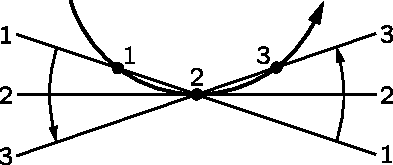
\includegraphics[width=0.8\linewidth]{fyz_fig405.pdf}
      \caption{Tři postupné pohledy na radiálně se pohybující bod na otáčející se podložce
              (\cite[s.~269]{Feynman01})}
      \label{fyz:fig405}
    \end{figure}

    Odvoďme vzorec pro Coriolisovu sílu, abychom viděli, jak skutečně působí. Předpokládejme, že
    Pavel sedí na rotující desce, která se mu zdá být nehybnou. Ale z hlediska Petra, který stojí na
    Zemi a zná správné zákony mechaniky, se deska otáčí. Předpokládejme, že jsme na desku nakreslili
    nějakou radiální přímku a že Pavel podél ní posouvá nějaké těleso. Chtěli bychom ukázat, že k
    tomu je potřebná boční síla. Podaří se nám to tak, když si všimneme momentu hybnosti tělesa.
    Těleso se točí se stálou úhlovou rychlostí \(\omega\), takže moment hybnosti je
    \begin{equation*}
      L=mv_{tang}r=mωr⋅r=mωr^2.
    \end{equation*}
    je-li tedy těleso blízko osy, má relativně malý moment hybnosti. Přesuneme-li ho do nové,
    vzdálenější polohy, zvětšíme \(r\), má těleso větší moment hybnosti. Má-li se pohybovat podél
    poloměru, musí na něj \emph{působit moment síly}. (Při chůzi podél poloměru po rotující desce je
    třeba se naklonit, působit silou na stranu. Někdy si to zkuste.) Potřebný moment síly je roven
    rychlosti změny \(L\) podle času, jak se těleso pohybuje podél poloměru. Jestliže se těleso
    pohybuje jen podél poloměru, \(\omega\) zůstává konstantní, takže moment síly je roven    
    \begin{equation*}
      τ=F_cr=\diff{L}{t}=\diff{(mωr^2)}{t}=2mωr\diff{r}{t},
    \end{equation*}
    kde \(F_c\) je \textbf{Coriolisova síla}. Chceme vědět, jakou boční sílu musí Pavel vynaložit,
    aby se těleso pohybovalo rychlostí \(v_r=\diff{r}{t}\). Je to síla \(F_c =\frac{N}{r}=2m\omega
    v_r\).
    
    Teď, když už máme vzorec pro Coriolisovu Sílu, se podívejme na celou situaci trochu podrobněji,
    abychom viděli, zda můžeme pochopit původ této síly z elementárnějšího hlediska. Všimněme si, že
    Coriolisova síla je stejná pro každý poloměr a je tedy přítomna dokonce i v počátku na ose
    otáčení! Ale vznik této síly v počátku lze zvlášť snadno pochopit, podíváme-li se na to, co se
    děje, z inerciální soustavy Petra, který stojí na zemi. Obr. \ref{fyz:fig405} znázorňuje tři
    postupné pohledy na pohyb bodu \(m\) procházejícího počátkem. Vidíme, že v důsledku rotace se
    bod nepohybuje po přímce, ale po \emph{zakřivené čáře}, jež se dotýká průměru desky v bodě
    \(r=0\). Aby se bod pohyboval po křivce, musí na něj působit síla, která mu dodává zrychlení v
    absolutním prostoru. To je Coriolisova síla.
    
    Coriolisova síla se objevuje i v jiných situacích. Můžeme ukázat, že i při pohybu tělesa
    konstantní rychlostí po obvodu kruhu na něj působí Coriolisova síla. Proč? Pavel vidí, že těleso
    se pohybuje po kružnici rychlostí \(v'\), z druhé strany Petr pozoruje rychlost \(v = v' + ωr\),
    neboť bod \(m\) je unášen deskou. Proto víme, čemu je síla skutečně rovna, konkrétně celkové
    odstředivé síle v důsledku rychlosti v, tj. \(mv^2/r\). Z Pavlova hlediska má odstředivá síla
    tři části. Můžeme je napsat následujícím způsobem
    

    
  \section{Příklady a cvičení}\label{fyz:IchapXIXsecV}

%---------------------------------------------------------------------------------------------------